\documentclass{amsart}
\usepackage{graphicx} % new way of doing eps files
\usepackage{listings} % nice code layout
\usepackage[usenames]{color} % color
\definecolor{listinggray}{gray}{0.9}
\definecolor{graphgray}{gray}{0.7}
\definecolor{blue}{rgb}{0,0,1}
\definecolor{green}{rgb}{0,0.6,0}
% \SciLab{title}{label}{file}
\newcommand{\SciLab}[3]{
  \lstset{language=Scilab}
  \lstset{backgroundcolor=\color{listinggray},rulecolor=\color{blue}}
  \lstset{linewidth=\textwidth}
  \lstset{commentstyle=\textit, stringstyle=\upshape,showspaces=false}
  \lstset{frame=tb}
  \lstinputlisting[caption={#1},label={#2}]{#3}
}
\lstdefinelanguage{JavaScript}{
  keywords={typeof, new, true, false, catch, function, return, null, catch, switch, var, if, in, while, do, else, case, break},
  keywordstyle=\color{blue}\bfseries,
  ndkeywords={class, export, boolean, throw, implements, import, this},
  ndkeywordstyle=\color{graphgray}\bfseries,
  identifierstyle=\color{black},
  sensitive=false,
  comment=[l]{//},
  morecomment=[s]{/*}{*/},
  commentstyle=\color{green}\ttfamily,
  stringstyle=\color{red}\ttfamily,
  morestring=[b]',
  morestring=[b]"
}
\lstset{
   language=JavaScript,
   backgroundcolor=\color{listinggray},
   extendedchars=true,
   basicstyle=\footnotesize\ttfamily,
   showstringspaces=false,
   showspaces=false,
   numbers=left,
   numberstyle=\footnotesize,
   tabsize=2,
   breaklines=true,
   showtabs=false,
   captionpos=b
}

\author{Cory Cook}
\title{Final Project}
\begin{document}
\maketitle
\tableofcontents
\section{Introduction}
The internet is a tool that is used by a third of the world's population. It allows us to connect and exchange information, provide services, and exchange ideas. The only problem is that in order to connect all of these devices and servers we need to lay out miles of wire and provide hubs that connect all of these wires together. Since most of us don't want to lay out the wires needed nor do we want to be responsible for managing the routers that connect all of these devices we need to have companies do this for us. Companies are happy to do this for us, for a modest fee. This turns out to be a bad deal for the customer as we are usually very limited to which internet service providers are available in the area, and, as such, those internet service providers have a lot of control over pricing and the quality of the services offered. Wouldn't it be better if we could do without the Internet Service Providers (ISPs) all together? In order to do this, however, we would need to be able to rid ourselves of our dependence on wires, routers, and other externally managed network focal points.

The goal of my final project is to provide a (very) basic implementation of a node-based networking system: including an addressing scheme, latency test, and speed test. Once I have a working implementation I will determine if the design is feasible by comparing it to modern internet tests and speeds offered by ISPs.
\section{Method}
I'm going to lay out the requirements of the design and then I'm going to abstract the requirements to better focus my solution to a general case, rather than a complete system. I'm going to ignore environmental and economic requirements and problems that would need to be considered as part of the design, and Im going to make false assumptions regarding the ethical use of the design by its users. Including such things would exceed the scope of the project and complicate the design beyond the problem I'm trying to solve.
\subsection{Requirements}
\begin{enumerate}
\item The system must allow connections to be established between any two devices on the network.
\item The system must allow data to be transferred from one device to another.
\item The system must not rely on any managed nodes or complicated systems that would require repair or maintenance.
\item The system must be extensible such that connections can be made over several different network types.
\item The system must be secure and data-safe.
\item The system must be able to forward data without recieving the entirety of the data (packets)
\end{enumerate}
\subsection{Abstraction}
For the purposes of this project I'm only going to consider the requirements necessary to establish connections and transfer data (1, 2, and 3). I'm also going to make several assumptions about the system that would not be true in a physical setting:
\begin{enumerate}
\item Assume all nodes are active. Nodes will not deactive throughout the duration of any transfers.
\item Assume all nodes are stationary. There will be no mobile nodes.
\item Assume that there is no data loss during transfer.
\item Assume that all nodes are techinically equivalent. All nodes will have the same properties (range, power, transfer rate, response time, etc.)
\item Assume that the devices can make an unlimitted number of concurrent connections.
\end{enumerate}
Given these abstractions I can create a relatively simple and expandable model that should be easy to implement.
\subsection{Design: Addressing Scheme}
The addressing scheme will have to be one such that a device will be able to contact another device on the network. In a network that doesn't have a cleary defined hierarchy, such as the one we are trying to implement, using a standard IP addressing scheme would not give the device enough information to know where to send its data. I'm sure that there are many solutions available to resolving addresses in a node-based network such as this. A couple of design solutions for addressing that I was able to come up with would work but each has its inefficiencies.

The first solution is to use a Global Positioning Satellite (GPS) Service to resolve addresses based on physical location. This would require the use of an external service that the device would have no control over. This GPS system would need to be actively maintained and serviced, which means that someone has to get paid. However, GPS services are currently being provided by the government so we are paying for it whether we like it or not. This does have the added benefit of being able to use the GPS coordinates to send data directly. Implementation of this would be relatively simple. Each device would poll a GPS system for its physical coordinates and build its address based on that. When the device needs to forward data it will forward the data to the device in the direction of the target system.

The second solution is to create a hierarchy by combining devices that are near each other. So a set of devices would represent a network group which would be contained within a larger group of groups, and so on until all devices are encompassed. Each device in the group would have addressing information for all devices within that group. This would be more difficult to implement as addressing would not be based on any kind of technology that already exists, and each device would need to have a lot more information and do a lot more calculation to resolve addressing for all requests. However, it does have the added benefit of not having to rely on any external system that would require regular maintenance. Implementation of this scheme would be more difficult than the first, expecially for optimization. Addressing would be based on levels, each level would contain a set number of devices or groups within it and assign an address for that group at that level. This could result in some very long addresses. When the device needs to forward data it will forward it outwards to all devices or groups until there is a match at that level.

For the purposes of this project I am going to implement the first solution, as it is much simpler. I am going to assume that the GPS system is a free service that is already in place. Each device on the network will be able to resolve its own address. I'm going to assume that the GPS has a high enough accuracy to give each device its own unique address. In a real-world situation there would be devices that fall within the same GPS coordinates and the system would have to account for that by adding the ability to select a specific device within an address or by expanding the address itself to fit a device-specific element. Either way it involves added complexity in device selection that, while being very closely related to this project, can be abstracted to get to (what I believe to be) the true goal of this project. That is to compare theoretical performance of this system to the high-maintenance systems currently being used. So I'm going to abstract this by assuming that each coordinate will have, at most, a single device. I'm going to abstract this further by not using true GPS coordinates and instead define the area of my test and randomly place objects within that area. Using true GPS would create very large addresses with very little meaning in the actual testing.
\subsection{Design: Performance Testing}
The performance of these systems can be determined through analysis of the specifications of the nodes, the relative distance between the client and the host, and the distance between each of the nodes. In order to analyze the performance between the design and currently used systems we must first be able to determine the best method for transferring data in the  system that we attempting to design. Once I have my emulated devices I am going to simulate data transfer as a function of the specification, analyze my data set to find the worst case scenario for my test area, and use the result to compare with current internet speed standards.
\subsection{Node Device Specifications}
\begin{description}
\item[Data Transfer Rate]Gigabit
\item[Maximum Range]40 meters
\item[Signal Degredation Rate]$\sqrt{-{{x-40}\over40}}$
\end{description}
The Data Transfer Rate is the rate of data transfer within the optimum range. The maximum range is the maximum distance in which a connection can be established.

These specifications were selected to ensure that the entire area of the next address over would be within optimum range for an addressing range of 8m regardless of the current position of the object within its own address range. 
\subsection{Implementation Description}
Each node is going to be an object with an address and a physical position. If the current address is (a,b) and the target address is (c,d) then the next address down the line will be determined by the following function (one-dimension):
\begin{equation}
a=c?a:a+{{c-a}\over{|c-a|}}
\end{equation}
We need to determine the physical distance between the nodes such that we can determine the signal strength and throughput. The throughput of the system is determined by the slowest data transfer on the line so if the bandwidth of the current node is less that that of the system throughput then set the system throughput as the current. Add any delay or latency incurred at the current node. Repeat until we reach the destination.

This should give us a latency and a throuput for a connection which is all we need to determine its performance. I will repeat this method for many random connections and record the data. Once I have the data I will determine a function that fits the given data and use optimization technique to find the worst case scenario for the system. Once this is determined I will compare the performance to the performance of the average internet users' connection and determine (roughly) if having a massive mesh networking system would be feasible.
\section{Implementation}
\SciLab{Mesh Network Implementation}{Performance Analysis}{set_val.sci}
\begin{figure}
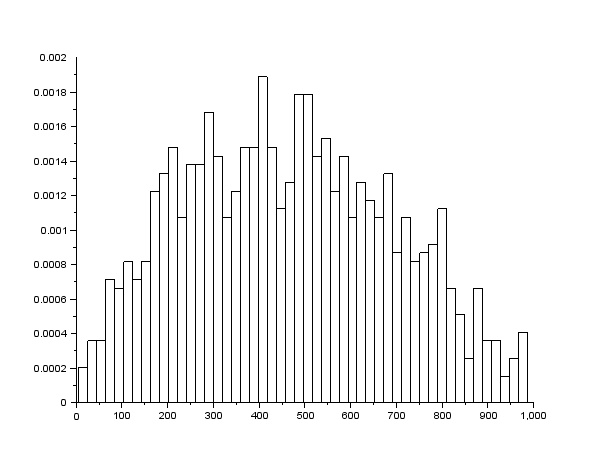
\includegraphics[width=400px]{latency_hist.jpg}
\caption{Latency Histogram Distribution vs. Time (ms)}
\end{figure}
\begin{figure}
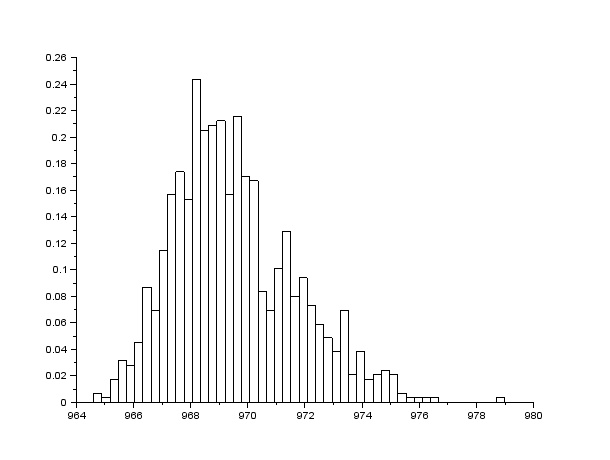
\includegraphics[width=400px]{bandwidth_hist_1000.jpeg}
\caption{Bandwidth Histogram @ Gigabit Distribution vs Speed (Mbps)}
\end{figure}
\begin{figure}
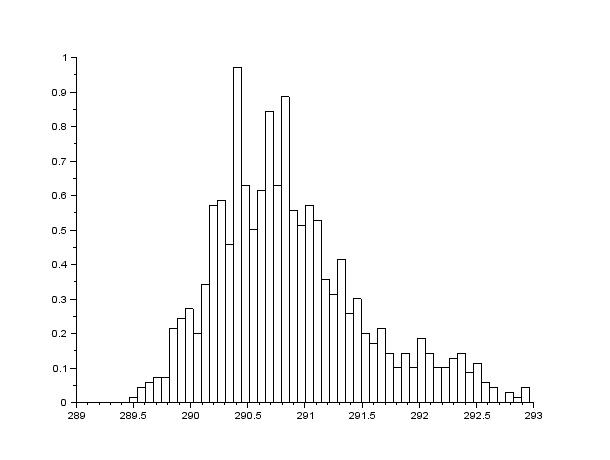
\includegraphics[width=400px]{bandwidth_hist_300.jpg}
\caption{Bandwidth Histogram @ 300 Mbps Distribution vs Speed (Mbps)}
\end{figure}
\begin{figure}
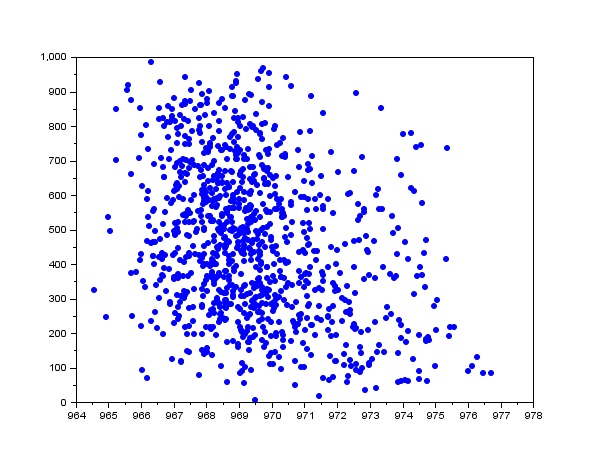
\includegraphics[width=400px]{bandwidth_latency_plot.jpg}
\caption{Bandwidth(Mbps) vs. Latency(ms)}
\end{figure}
\section{Conclusion}
The data shows that given the test area of $64 km^2$ the current implementation of the wireless mesh network would be infeasible due to high latency. However, there is a large improvement in bandwidth over the average high-speed internet available via ISP, which currently averages about 30 Mbps.

This is a very abstract model of a simple implementation of a mesh network. A complete mesh network would be able to determine the best node to forward the data to based on the situation. It would also be able to send data to multiple nodes to ensure delivery or improve performance.

The charts show that Bandwidth and Latency are not directly correllated. This means that an effect in the latency does not guarantee an effect in the bandwidth and the only real factors are the distance between the nodes and the number of nodes transversed. Theoretically, although not supported by my charts, bandwidth and latency are correllated because selecting nodes that are further away would reduce the number of nodes necessary and, therefore, improve latency. On the other hand, choosing nodes that are closer would close the distance between nodes and, therefore, improve the bandwidth between the nodes. So distance between nodes affects both latency and bandwidth.

I would like to move in the direction of a self-managed networking system similar to the one modelled here. This would allow us to move away from the shackles of ISPs and Data Carriers and implement network capability into nearly all devices. Cars would be able to talk to each other freely to prevent accidents and improve road safety, data would be available to you from almost any device at nearly any location, lost devices and people could easily be tracked and found, the benefits are limitless and all without having to pay hundreds of dollars for the privilege to access them.
\end{document}